\section{Motivating Examples}
\label{sec:motiv}

We begin our motivation for a tool such as \app by providing several misconfiguration examples, and showing how do we address them. All these examples are extracted from real-world reports%
~\cite{yin11anempirical, configdataset}. When writing configuration files, the user usually takes already existing files and modifies them. If the original file is already corrupted, the errors are propagated further. However, even if the original file is correct, changing the file by a non-expert user can easily result in errors.


\subsection{Ordering Errors}

When configuring PHP to run with the Apache HTTP Server the user writes, among others, the following lines:\\
 \texttt{
 \hspace*{3em}extension = mysql.so\\
 \hspace*{3em}...\\
 \hspace*{3em}extension = recode.so}\\
This file caused that the Apache server could not start due to 
the segmentation fault error. Running \app on this file returns\\
 \texttt{
  one line output from our tool that indicates that things should be reordered}\\
Indeed, this was the source of the error. When using PHP in Apache, the
extension ``mysql.so'' depends on ``recode.so'' and the relative ordering 
of two of them is crucial. The user is informed that ``recode.so'' should appear before ``mysql.so''.

\subsection{Entry Missing Errors}

If the user wants to use OpenLDAP to enable her directory access
protocol, she needs to use the password policy overlay. This is usually
done through the following entries in the OpenLDAP configuration file:\\
\texttt{
 \hspace*{3em}overlay ppolicy\\}
However, this configuration file will make LDAP server fail to work.
Running \app on this configuration file returns:
\xxx{Mark, put results here}\\
This was the source of the error. When using the password policy overlay
in OpenLDAP, we have to first include the related schema. The correct configuration should be:\\
\texttt{
 \hspace*{3em}include schema/ppolicy.schema\\
 \hspace*{3em}overlay ppolicy\\
}

\subsection{Value Type Errors}

If the user tries to install MySQL, she first needs to 
initiate the path for the
log information generated by MySQL. A user puts the following code in 
her MySQL configuration file:\\
\texttt{
 \hspace*{3em}general\_log = /var/log/mysql/mysql.log\\}
Unfortunately, the log information cannot be correctly written.
After \app analyzed this configuration file, it correctly identifies the error:
\xxx{Mark, put results here}\\
The entry ``general\_log'' should be an integer, 
and not a string. In MySQL, there is another entry named
``general\_log\_file'' which is used to specify the log path.  

\subsection{Value Correlation Errors}

When configuring PHP on MySQL, the user writes the following lines 
of entries in her both PHP and MySQL configuration files:\\
\texttt{
 \hspace*{3em}mysql's config\\
 \hspace*{3em}max\_connections = 300\\
 \hspace*{3em}...\\
 \hspace*{3em}php's config\\
 \hspace*{3em}mysql.max\_persistent = 400\\}
This will cause MySQL to abort with the error information:
``too many connections''.
Running \app on this combined configuration file returns:
\xxx{Mark, put results here}\\
We are successfully able to derive arithmetic relations between integer values.
In particular, the ``mysql.max\_persistent'' in PHP should be no
larger than the ``max\_connections'' in MySQL configuration file.

\subsection{Format Errors}
\xxx{I am not sure if we still need the format error, so I 
put it the last one.}

When configuring NetApp commercial storage system, 
the user writes the following entry:\\
\texttt{
 \hspace*{3em}InitiatorName: iqn:DEV\_DOMAIN\\
} 
The NetApp storage share cannot be recognized. 
Thus, we run \app on this configuration file and get the results:
\xxx{Mark, put results here}\\
This is the root-cause of the problem,
since the iscsi device's initiator name, \ie, InitiatorName,
only allows lowercase letters. However, the user sets the name with
capital letters ``DEV\_DOMAIN''.

\com{
\begin{figure}[t] \centering
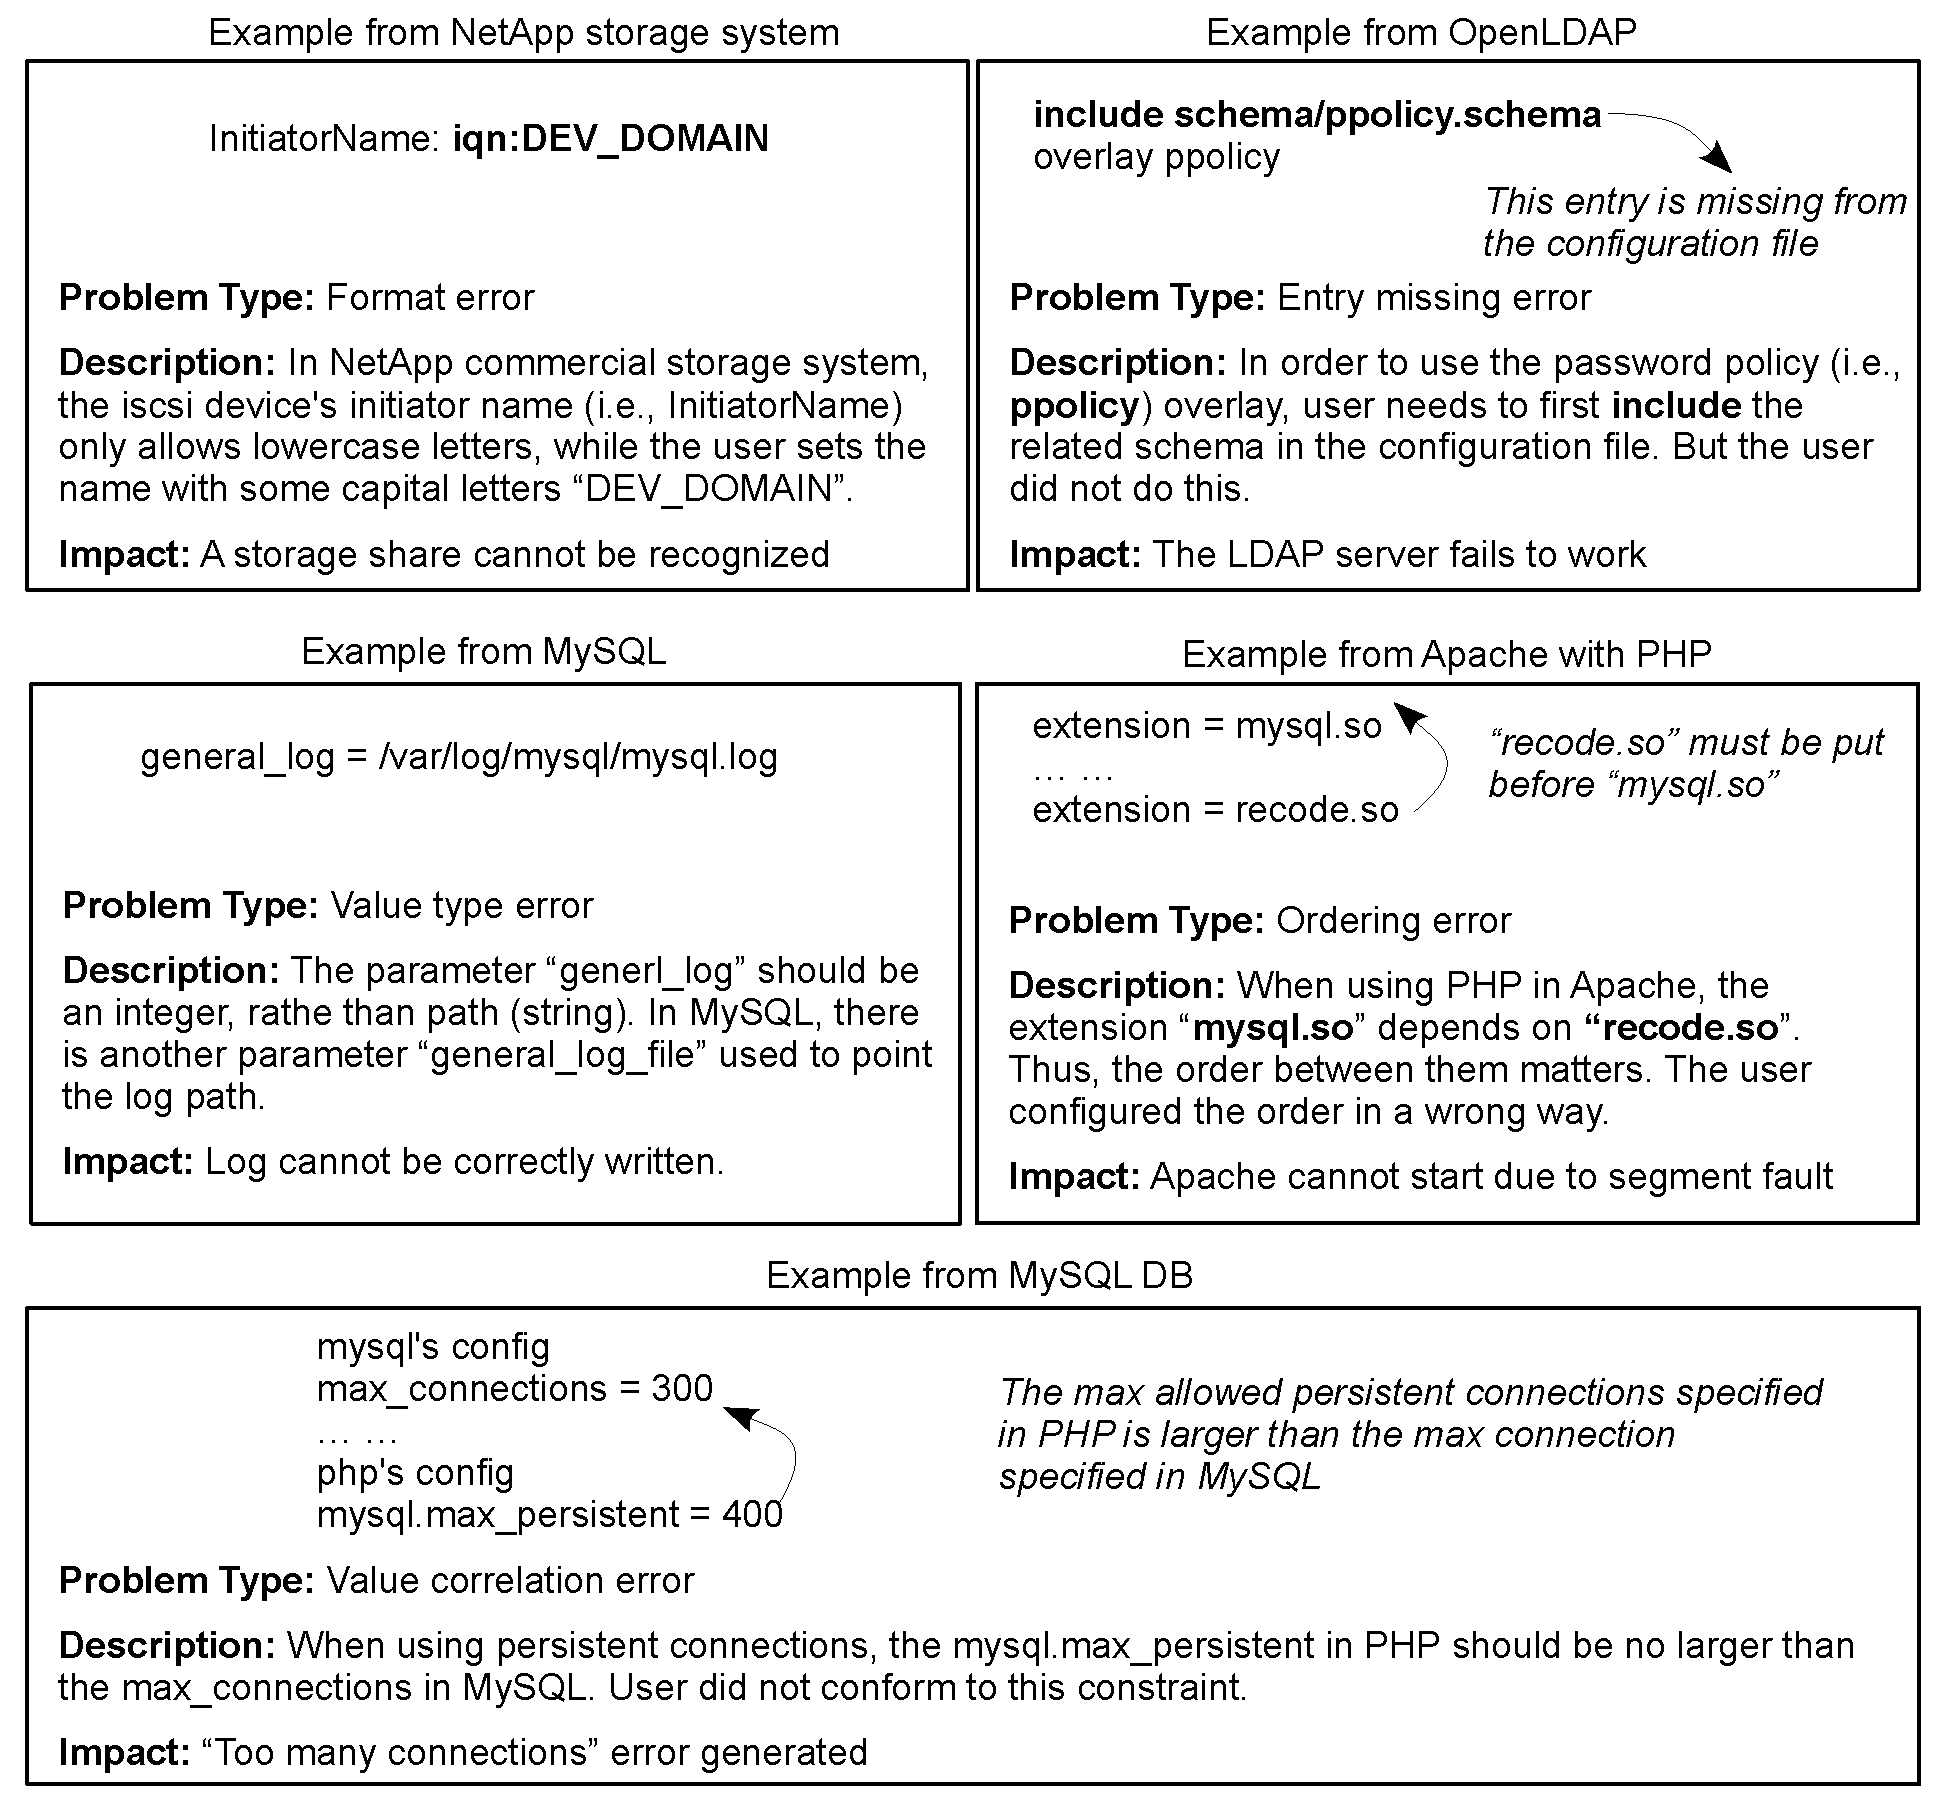
\includegraphics[width=0.98\textwidth]{figs/example}
\caption{Motivating examples. Our target configuration errors are
  classified into five groups. The five examples here correspond to
  these groups, respectively.}
\label{fig-example}
\end{figure}

Fig.~\ref{fig-example} presents misconfiguration examples in real-world
that we aim to address. All the examples are extracted from
misconfiguration issues reported in real-world efforts%
~\cite{yin11anempirical, configdataset}.
We classify our target configuration errors
into five groups: 1) format error; 2) entry missing error; 3) value type
error; 4) ordering error; and 5) value correlation error.
The five examples in Fig.~\ref{fig-example} correspond to the above five
groups, respectively.

} 
